\documentclass[../document.tex]{subfiles}
\begin{document}\label{ssec:energy}

\begin{figure*}[htb]
\begin{subfigure}{.49\textwidth}
\centering
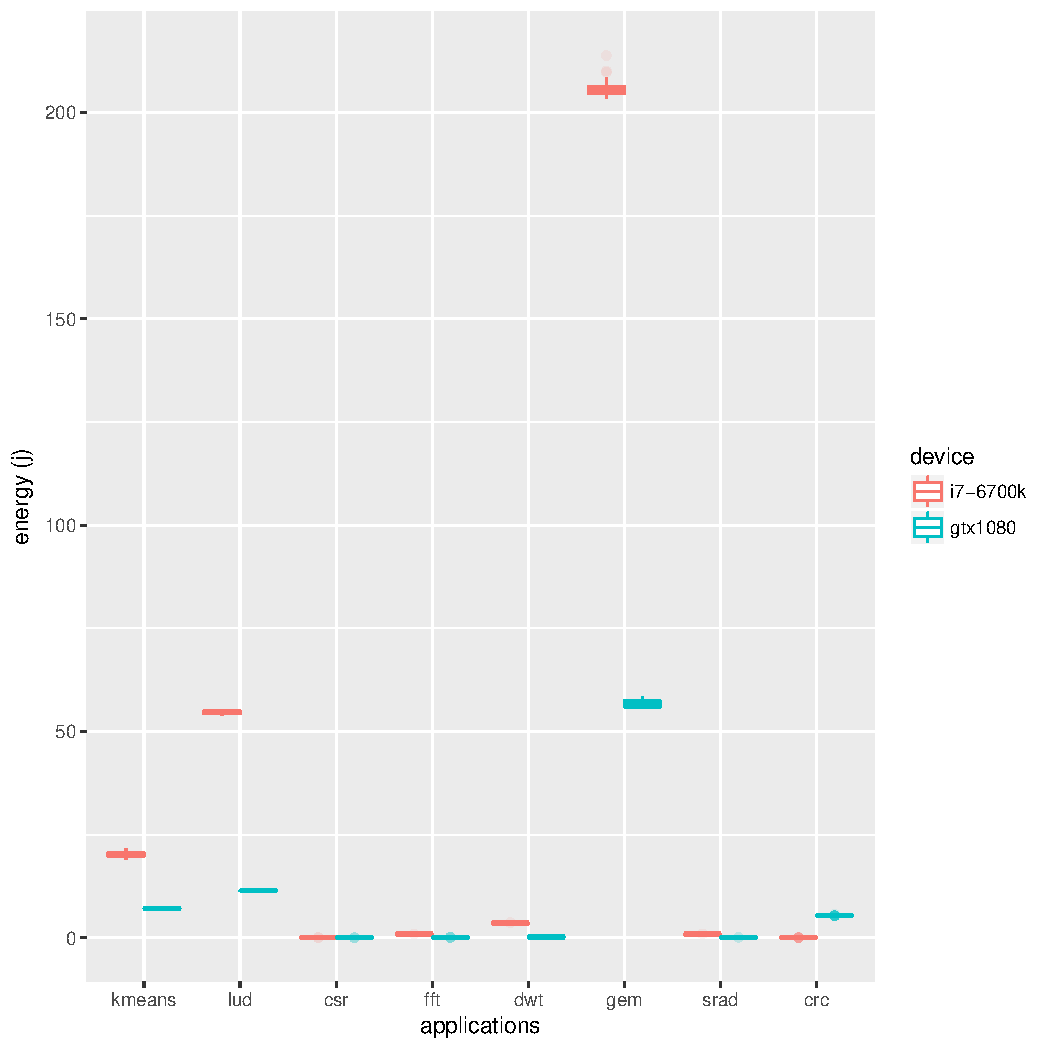
\includegraphics[width=1\textwidth]{figures/energy-results/energy_charts.pdf}
\caption{Kernel execution energy}
\label{fig:energy}
\end{subfigure}
\hfill
\begin{subfigure}{.49\textwidth}
\centering
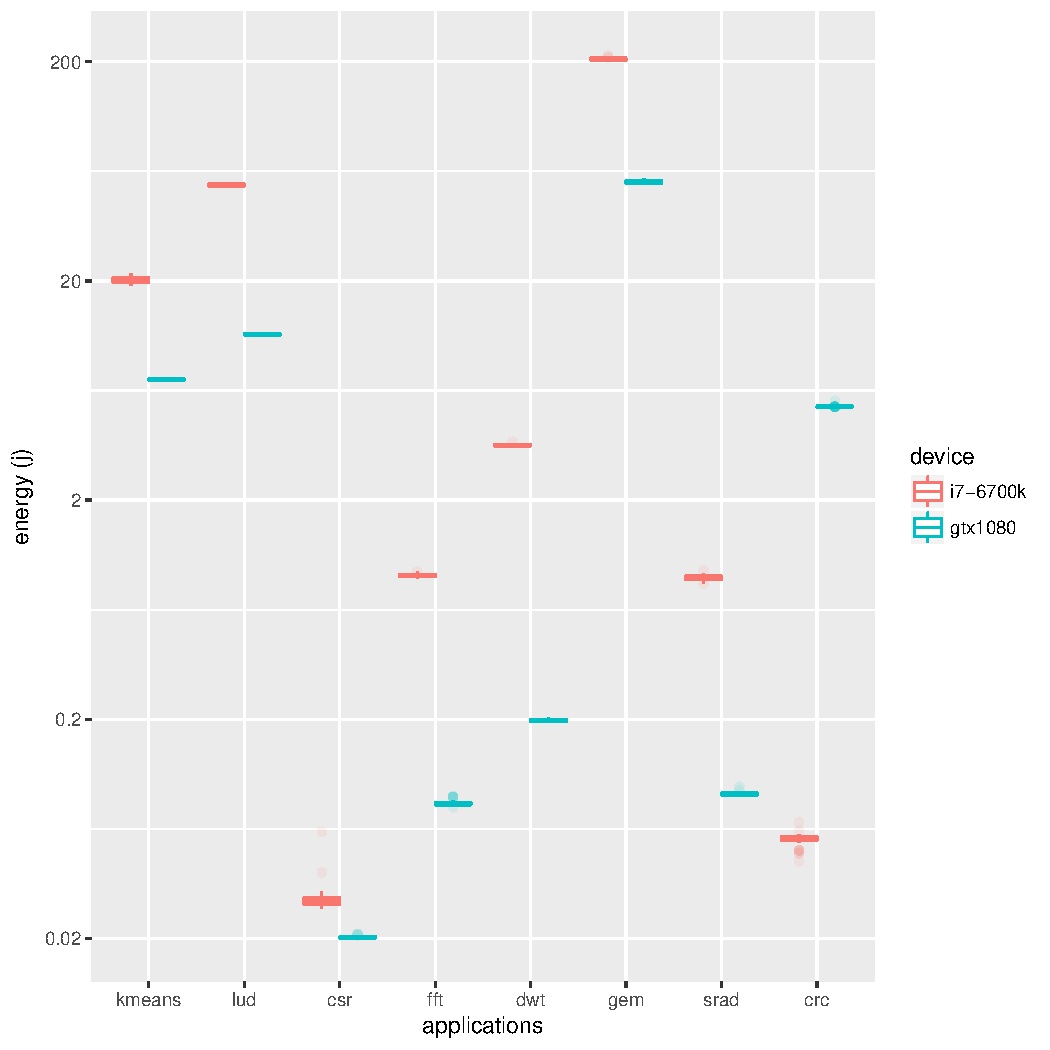
\includegraphics[width=1\textwidth]{figures/energy-results/energy_charts_log10.pdf}
\caption{Log of kernel execution energy}
\label{fig:energy-log}
\end{subfigure}
\caption{Energy requirement for kernel execution for each benchmark on Core i7-6700K and Nvidia GTX1080}
\end{figure*}

\todo{Does energy scale with problem size for all benchmarks? Maybe not since dwarfs with large memory access cache misses could add huge overheads}

From the time results presented in Section~\ref{ssec:time} we see the largest difference occurs between CPU and GPU type accelerators at the {\bf large} problem size.
Thus we expect that the {\bf large} problem size will also show the largest difference in energy.
This is explored in Figures~\ref{fig:energy} and~\ref{fig:energy-log} where several benchmarks are compared over the {\bf large} size.
All results are presented in joules.
Each pair of box plots has been grouped by colour according to device, red for the Intel Skylake i7-6700k CPU and blue for the Nvidia GTX1080 GPU.
These were the only devices examined since collection of RAPL and NVML PAPI performance measurements (with LibSciBench) requires super user access, and both these devices were the only accelerators available with this permission.
Nonetheless, certain trends become apparent when directly comparing joules required over a range of problems.
The logarithmic transformation has been applied to Figure~\ref{fig:energy-log} to emphasise the variation at smaller energy scales (< \SI{1}{\joule}), which was necessary due to small execution times for some benchmarks.
In future this will be addressed by balancing the amount of computation required for each benchmark, to standardize the magnitude of results.

The distributions were collected by measuring solely the kernel execution over a distribution of 50 runs.
Variance with respect to energy usage is larger on the CPU, which is consistent with the execution time results.

\end{document}
